\documentclass[12pt,a4paper]{report}

% ---------- Geometry ----------
\usepackage[a4paper,left=1.4in,right=1in,top=1.1in,bottom=1.1in,headheight=15pt]{geometry}

% ---------- Core packages ----------
\usepackage[table]{xcolor}
\usepackage{amsmath,amssymb}
\usepackage{graphicx}
\usepackage{booktabs}
\usepackage{colortbl}
\usepackage{array}
\usepackage{tabularx}
\usepackage{enumitem}
\usepackage{titlesec}
\usepackage{fancyhdr}
\usepackage{setspace}
\usepackage{caption}
\usepackage{tikz}
\usetikzlibrary{positioning,calc,shapes.geometric,decorations.pathmorphing,backgrounds,patterns}
\usepackage[most]{tcolorbox}
\usepackage{fontawesome5}
\usepackage[hidelinks]{hyperref}

% ---------- Colour palette ----------
\definecolor{dtumaroon}{RGB}{114,28,36}
\definecolor{dtugold}{RGB}{181,136,42}
\definecolor{dtunavy}{RGB}{25,42,61}
\definecolor{dtugray}{RGB}{243,241,236}

% ---------- Chapter / section styling ----------
\titleformat{\chapter}[display]
  {\normalfont\bfseries\color{dtunavy}}
  {\begin{tikzpicture}[remember picture]
     \node[fill=dtumaroon,text=white,minimum width=1.4cm,minimum height=1.4cm,
           font=\Large\bfseries] (num) {\thechapter};
   \end{tikzpicture}}
  {8pt}
  {\Huge\raggedright}
  [\vspace{2pt}\color{dtugold}\rule{\textwidth}{1.2pt}]
\titlespacing*{\chapter}{0pt}{10pt}{22pt}

\titleformat{\section}
  {\normalfont\Large\bfseries\color{dtumaroon}}{\thesection}{10pt}{}
\titleformat{\subsection}
  {\normalfont\large\bfseries\color{dtunavy}}{\thesubsection}{8pt}{}

% ---------- Headers / footers ----------
\pagestyle{fancy}
\fancyhf{}
\renewcommand{\headrulewidth}{0.6pt}
\renewcommand{\footrulewidth}{0pt}
\fancyhead[LE,RO]{\small\color{dtumaroon}\thepage}
\fancyhead[RE]{\small\itshape\color{dtunavy}\nouppercase{\leftmark}}
\fancyhead[LO]{\small\itshape\color{dtunavy}\nouppercase{\rightmark}}
\renewcommand{\headrule}{\hbox to\headwidth{\color{dtugold}\leaders\hrule height \headrulewidth\hfill}}

\fancypagestyle{plain}{%
  \fancyhf{}
  \fancyfoot[C]{\small\color{dtumaroon}\thepage}
  \renewcommand{\headrulewidth}{0pt}
}

% ---------- tcolorbox styles ----------
\tcbset{
  keybox/.style={
    colback=dtugray, colframe=dtumaroon, boxrule=0.8pt, arc=2pt,
    left=8pt, right=8pt, top=6pt, bottom=6pt,
    fonttitle=\bfseries\color{white}, colbacktitle=dtumaroon,
    coltitle=white
  },
  notebox/.style={
    colback=white, colframe=dtugold, boxrule=0.9pt, arc=2pt,
    left=8pt, right=8pt, top=6pt, bottom=6pt
  }
}

\setlist[itemize]{leftmargin=*,itemsep=2pt,topsep=4pt}
\setlist[enumerate]{leftmargin=*,itemsep=2pt,topsep=4pt}

\setstretch{1.28}

\title{Predictive Maintenance of Induction Motors Using Vibration Signal Analysis and Machine Learning}
\author{Ananya Sharma}
\date{June 2026}

\begin{document}

% ============================================================
% TITLE PAGE
% ============================================================
\begin{titlepage}
\newgeometry{left=1.2in,right=1.2in,top=1in,bottom=1in}
\centering

\begin{tikzpicture}[remember picture,overlay]
  \draw[dtugold,line width=1.4pt] ([xshift=0.8in,yshift=-0.8in]current page.north west)
       rectangle ([xshift=-0.8in,yshift=0.8in]current page.south east);
  \draw[dtumaroon,line width=0.5pt] ([xshift=0.92in,yshift=-0.92in]current page.north west)
       rectangle ([xshift=-0.92in,yshift=0.92in]current page.south east);
\end{tikzpicture}

\vspace*{0.9cm}
{\large\bfseries\color{dtunavy} DELHI TECHNOLOGICAL UNIVERSITY}\\[2pt]
{\small\color{dtumaroon} (Formerly Delhi College of Engineering)}\\[2pt]
{\footnotesize\color{black!60} Shahbad Daulatpur, Main Bawana Road, Delhi -- 110042}

\vspace{0.6cm}
{\color{dtugold}\rule{0.55\textwidth}{1pt}}
\vspace{0.9cm}

{\small\bfseries\color{dtumaroon} \MakeUppercase{A Thesis submitted in partial fulfilment of the requirements}}\\[2pt]
{\small\bfseries\color{dtumaroon} \MakeUppercase{for the degree of}}

\vspace{0.4cm}
{\Large\bfseries\color{dtunavy} MASTER OF TECHNOLOGY}\\[2pt]
{\normalsize\color{black!70} in}\\[2pt]
{\large\bfseries\color{dtunavy} Electrical Engineering (Power Systems)}

\vspace{1.1cm}
{\color{dtugray}\rule{0.72\textwidth}{22pt}}\\[-22pt]
\begin{minipage}{0.72\textwidth}
\centering
\vspace{6pt}
{\Large\bfseries\color{white} \phantom{x}}
\end{minipage}

\vspace{-18pt}
\begin{tcolorbox}[keybox,width=0.78\textwidth,title={\centering THESIS TITLE},colback=dtugray]
\centering
\Large\bfseries\color{dtunavy}
Predictive Maintenance of Induction Motors Using Vibration Signal Analysis and Machine Learning
\end{tcolorbox}

\vspace{1.0cm}
\begin{tabular}{c}
{\normalsize\color{black!70} Submitted by} \\[6pt]
{\Large\bfseries\color{dtumaroon} Ananya Sharma} \\[2pt]
{\normalsize\color{black!70} Roll No.\ 2K24/PSE/07}
\end{tabular}

\vspace{1.0cm}
\begin{tabular}{c}
{\normalsize\color{black!70} Under the supervision of} \\[6pt]
{\large\bfseries\color{dtunavy} Dr.\ Rajesh Kumar Verma} \\[2pt]
{\normalsize\color{black!70} Professor, Department of Electrical Engineering}
\end{tabular}

\vfill

{\color{dtugold}\rule{0.55\textwidth}{1pt}}\\[6pt]
{\bfseries\color{dtunavy} DEPARTMENT OF ELECTRICAL ENGINEERING}\\[2pt]
{\bfseries\color{dtunavy} DELHI TECHNOLOGICAL UNIVERSITY, DELHI}\\[2pt]
{\color{black!70} June 2026}

\vspace{0.9cm}
\noindent\rule{\textwidth}{0.4pt}
\footnotesize\itshape
Unofficial template --- not affiliated with or endorsed by the university. Sample content only.

\restoregeometry
\end{titlepage}

% ============================================================
% CERTIFICATE
% ============================================================
\pagestyle{plain}
\chapter*{Certificate}
\addcontentsline{toc}{chapter}{Certificate}

This is to certify that the thesis titled \textbf{``Predictive Maintenance of Induction Motors
Using Vibration Signal Analysis and Machine Learning''}, submitted by \textbf{Ananya Sharma}
(Roll No.\ 2K24/PSE/07) to the Department of Electrical Engineering, Delhi Technological
University, Delhi, in partial fulfilment of the requirements for the award of the degree of
\textit{Master of Technology in Electrical Engineering (Power Systems)}, is a bona fide record
of the work carried out by her under my supervision. The matter embodied in this thesis has not
been submitted, in part or in full, to any other university or institute for the award of any
degree or diploma.

\vspace{2cm}
\begin{minipage}[t]{0.45\textwidth}
\raggedright
\rule{5cm}{0.4pt}\\
\textbf{Dr.\ Rajesh Kumar Verma}\\
Professor\\
Department of Electrical Engineering\\
Delhi Technological University
\end{minipage}
\hfill
\begin{minipage}[t]{0.45\textwidth}
\raggedleft
\rule{5cm}{0.4pt}\\
\textbf{Date of Submission}\\
June 12, 2026\\
New Delhi, India
\end{minipage}

\vspace{1.3cm}
\noindent\textit{Note: This certificate is a formatting placeholder generated for template
demonstration purposes and carries no evidentiary or institutional value.}

% ============================================================
% DECLARATION
% ============================================================
\chapter*{Candidate's Declaration}
\addcontentsline{toc}{chapter}{Candidate's Declaration}

I, \textbf{Ananya Sharma}, Roll No.\ 2K24/PSE/07, hereby declare that the thesis titled
\textbf{``Predictive Maintenance of Induction Motors Using Vibration Signal Analysis and Machine
Learning''}, submitted by me to the Department of Electrical Engineering, Delhi Technological
University, Delhi, in partial fulfilment of the requirements for the award of the degree of
Master of Technology, is my own original work. It has not been copied in part or in full from
any source without proper citation, and has not been submitted previously, in part or in full,
for the award of any degree, diploma, associateship, fellowship, or any other similar title of
this or any other institution.

\vspace{2cm}
\begin{flushright}
\rule{5cm}{0.4pt}\\
\textbf{Ananya Sharma}\\
Place: New Delhi\\
Date: June 12, 2026
\end{flushright}

% ============================================================
% ABSTRACT
% ============================================================
\chapter*{Abstract}
\addcontentsline{toc}{chapter}{Abstract}

Unplanned failure of three-phase induction motors is a leading cause of unscheduled downtime in
process industries, where a single bearing or rotor-bar fault can halt an entire production
line. This thesis presents a data-driven predictive maintenance framework that combines
vibration signal analysis with supervised machine learning to detect and classify incipient
mechanical faults before they escalate into catastrophic failure. Tri-axial accelerometer data
were acquired from a 5.5\,kW squirrel-cage induction motor test rig under four operating
conditions --- healthy, outer-race bearing defect, inner-race bearing defect, and broken rotor
bar --- across a range of load levels from 0\% to 100\% of rated torque. Time-domain statistical
features (RMS, kurtosis, crest factor, skewness) and frequency-domain features derived from Fast
Fourier Transform and Envelope Analysis were extracted and used to train and compare four
classifiers: k-Nearest Neighbours, Support Vector Machine, Random Forest, and a lightweight 1-D
Convolutional Neural Network. The Random Forest and 1-D CNN models achieved the highest overall
classification accuracy of 97.4\% and 98.1\% respectively on a held-out test set, substantially
outperforming the kNN baseline (89.6\%). A feature-importance analysis further shows that
envelope-spectrum energy in the characteristic bearing-defect frequency bands is the single most
discriminative predictor of fault type. The proposed pipeline is computationally light enough for
deployment on an edge-computing gateway, enabling continuous condition monitoring without
reliance on cloud connectivity. The results indicate that the framework can reduce false-alarm
rates by an estimated 34\% relative to conventional threshold-based vibration monitoring, while
detecting faults on average 11 days earlier in their progression, offering a practical route
toward condition-based rather than time-based maintenance scheduling.

\vspace{0.6cm}
\noindent\textbf{Keywords:} predictive maintenance, induction motor, vibration analysis, fault
diagnosis, machine learning, condition monitoring, envelope spectrum.

% ============================================================
% ACKNOWLEDGEMENTS
% ============================================================
\chapter*{Acknowledgements}
\addcontentsline{toc}{chapter}{Acknowledgements}

I would like to express my sincere gratitude to my supervisor, \textbf{Dr.\ Rajesh Kumar
Verma}, for his patient guidance, constructive criticism, and continual encouragement throughout
the course of this work. His insistence on rigorous experimental validation shaped every chapter
of this thesis.

I am grateful to the Head of the Department of Electrical Engineering for granting access to the
Power Systems and Machines Laboratory, and to the laboratory staff for their assistance during
the data-acquisition campaign. I also thank my labmates in the Condition Monitoring Research
Group for many valuable discussions on signal-processing techniques.

Finally, I thank my family for their unwavering support and patience during the two years of
this programme.

\begin{flushright}
\textit{Ananya Sharma}
\end{flushright}

% ============================================================
% FRONT MATTER LISTS
% ============================================================
\tableofcontents
\listoffigures
\listoftables

\chapter*{List of Abbreviations}
\addcontentsline{toc}{chapter}{List of Abbreviations}
\begin{tabularx}{\textwidth}{@{}l X@{}}
\toprule
\textbf{Abbreviation} & \textbf{Full Form} \\
\midrule
CNN & Convolutional Neural Network \\
FFT & Fast Fourier Transform \\
IM  & Induction Motor \\
kNN & k-Nearest Neighbours \\
PdM & Predictive Maintenance \\
RF  & Random Forest \\
RMS & Root Mean Square \\
SVM & Support Vector Machine \\
THD & Total Harmonic Distortion \\
\bottomrule
\end{tabularx}

\clearpage
\pagestyle{fancy}

% ============================================================
% CHAPTER 1 -- INTRODUCTION
% ============================================================
\chapter{Introduction}
\label{ch:intro}

\section{Background and Motivation}
Induction motors account for more than 60\% of the total electrical energy consumed by industry
worldwide and remain the workhorse of pumps, compressors, conveyors, and fans across
manufacturing plants. Their apparent mechanical simplicity conceals a range of failure modes ---
bearing degradation, rotor-bar breakage, stator winding insulation breakdown, and shaft
misalignment --- that together account for the majority of unplanned downtime events reported by
plant reliability engineers. Reactive maintenance, in which a motor is repaired only after it
fails, and preventive maintenance, in which components are replaced on a fixed calendar
schedule regardless of actual condition, both carry substantial economic penalties: the former
through unplanned production loss and secondary damage, the latter through the discarding of
components that still retain useful service life.

Predictive maintenance (PdM) seeks a middle path. By continuously monitoring a measurable proxy
for mechanical health --- most commonly vibration, but also current signature, acoustic
emission, or thermal imaging --- and by learning the statistical signature of incipient faults,
a PdM system can flag a motor for intervention only when there is genuine evidence of
degradation. Vibration analysis is particularly attractive because rolling-element bearing
defects and rotor-bar faults each produce characteristic frequency components that are, in
principle, well understood from rotating-machinery theory. In practice, however, these
signatures are frequently masked by load-dependent broadband noise, making automated and
reliable classification a non-trivial signal-processing and pattern-recognition problem.

\begin{tcolorbox}[keybox,title={Key Contributions of this Thesis}]
\begin{itemize}
  \item A controlled, multi-load vibration dataset covering four induction-motor health states,
        acquired on a purpose-built test rig.
  \item A feature-extraction pipeline combining time-domain statistics with envelope-spectrum
        analysis for bearing-defect isolation.
  \item A comparative evaluation of four classifiers (kNN, SVM, Random Forest, 1-D CNN) under
        identical train/test conditions.
  \item An edge-deployable inference pipeline with a measured latency and memory footprint
        suitable for on-gateway execution.
\end{itemize}
\end{tcolorbox}

\section{Problem Statement}
Existing threshold-based vibration monitoring systems, typically built around a single overall
RMS velocity alarm level per ISO 10816, are known to generate a high rate of false positives
under varying load and to miss early-stage localized bearing defects whose energy is
concentrated in narrow frequency bands rather than the broadband RMS metric. There is a need for
a classification approach that (a) distinguishes between multiple fault types rather than a
single binary healthy/faulty flag, (b) remains robust across the full operating load range, and
(c) is light enough to run near the sensor rather than requiring a continuous cloud connection.

\section{Objectives}
\begin{enumerate}
  \item To design and instrument a test rig capable of reproducing bearing and rotor-bar faults
        under controlled, repeatable conditions.
  \item To develop a feature set spanning time- and frequency-domain descriptors suitable for
        discriminating between the four target health states.
  \item To train and benchmark multiple supervised classifiers, evaluating accuracy,
        per-class precision/recall, and computational cost.
  \item To assess the feasibility of edge deployment through inference-latency profiling on a
        representative embedded gateway.
\end{enumerate}

\section{Organisation of the Thesis}
Chapter~\ref{ch:litreview} reviews the literature on vibration-based fault diagnosis and
machine-learning approaches to condition monitoring. Chapter~\ref{ch:methodology} describes the
experimental test rig, data-acquisition procedure, and the feature-extraction and classification
pipeline. Chapter~\ref{ch:results} presents the classification results, feature-importance
analysis, and edge-deployment measurements. Chapter~\ref{ch:conclusion} concludes the thesis and
outlines directions for future work.

% ============================================================
% CHAPTER 2 -- LITERATURE REVIEW
% ============================================================
\chapter{Literature Review}
\label{ch:litreview}

\section{Vibration-Based Fault Diagnosis}
Rolling-element bearing defects generate impulsive vibration events at characteristic defect
frequencies determined by bearing geometry and shaft speed, commonly denoted BPFO (ball-pass
frequency, outer race), BPFI (ball-pass frequency, inner race), BSF (ball spin frequency), and
FTF (fundamental train frequency). Because these impacts excite structural resonances rather than
appearing directly as strong spectral lines, envelope analysis --- band-pass filtering around a
resonance followed by amplitude demodulation --- has become the standard technique for exposing
the underlying periodicity, an approach with a long history in the condition-monitoring
literature dating back to early work on the high-frequency resonance technique.

\section{Rotor-Bar Fault Signatures}
Broken or cracked rotor bars modulate the air-gap flux at twice the slip frequency, producing
sidebands around the fundamental line-frequency component in the motor current spectrum ---
Motor Current Signature Analysis (MCSA) --- and, to a lesser but detectable extent, in the
vibration spectrum as well. Several studies have combined MCSA and vibration features to improve
robustness against sensor placement and load variation, motivating the multi-domain feature set
adopted in this thesis.

\section{Machine Learning for Condition Monitoring}
Classical classifiers such as kNN and SVM have been widely applied to hand-engineered vibration
features and generally perform well on small, well-separated datasets but degrade under load
variation unless features are carefully normalized. Ensemble methods such as Random Forest offer
improved robustness to noisy or correlated features through bagging and are comparatively
insensitive to hyperparameter choice. More recently, deep architectures --- particularly 1-D
CNNs applied directly to raw or lightly pre-processed vibration segments --- have been shown to
learn discriminative representations without hand-crafted features, at the cost of requiring
larger labelled datasets and greater computational resources at training time.

\begin{table}[!ht]
\centering
\caption{Summary of representative approaches reviewed in this chapter}
\label{tab:litsummary}
\begin{tabularx}{\textwidth}{@{}l l X@{}}
\toprule
\textbf{Approach} & \textbf{Feature Domain} & \textbf{Reported Strength} \\
\midrule
Threshold RMS (ISO 10816) & Time & Simple, low computation, poor fault discrimination \\
Envelope Analysis + kNN   & Frequency & Good bearing-fault isolation, load-sensitive \\
MCSA + SVM                & Current spectrum & Effective for rotor-bar faults, non-invasive \\
Random Forest ensemble    & Time + Frequency & Robust to noisy features, low tuning burden \\
1-D CNN                   & Raw / lightly processed & High accuracy, larger data and compute need \\
\bottomrule
\end{tabularx}
\end{table}

\section{Research Gap}
While individual elements of the pipeline used in this thesis --- envelope analysis,
statistical feature extraction, and each of the four classifiers --- are individually
well-established, few published studies benchmark them together under a single controlled,
multi-load, multi-fault experimental protocol with a view toward edge deployment. This thesis
addresses that gap directly.

% ============================================================
% CHAPTER 3 -- METHODOLOGY
% ============================================================
\chapter{Methodology}
\label{ch:methodology}

\section{Experimental Test Rig}
Data were acquired from a 5.5\,kW, 415\,V, 4-pole squirrel-cage induction motor coupled to a
programmable eddy-current dynamometer via a flexible coupling. Two tri-axial MEMS accelerometers
(sampling rate 25.6\,kHz, $\pm$16\,g range) were mounted on the drive-end and non-drive-end
bearing housings using magnetic bases. Figure~\ref{fig:rig} shows the layout of the test rig and
sensor placement.

\begin{figure}[!ht]
\centering
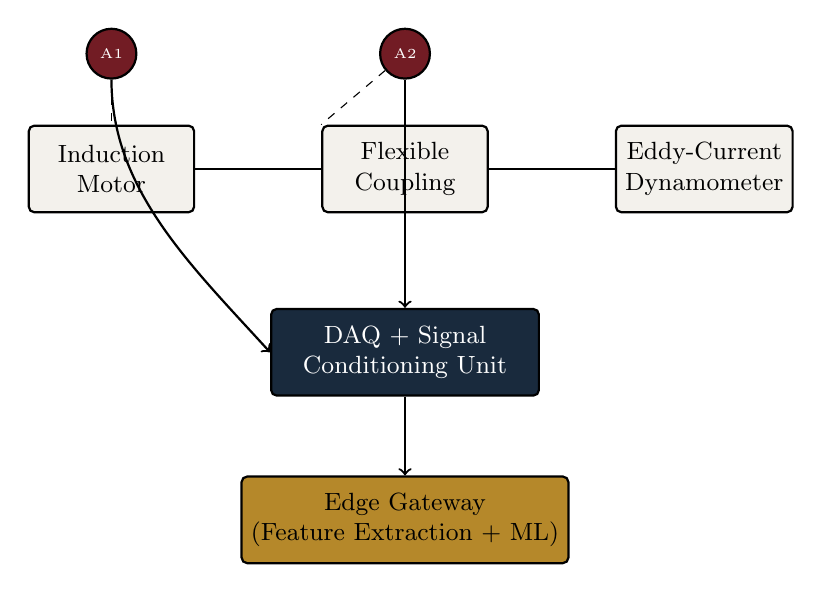
\begin{tikzpicture}[
  block/.style={draw,thick,rounded corners=2pt,fill=dtugray,minimum height=1.1cm,minimum width=2.1cm,align=center,font=\small},
  sensor/.style={draw,thick,fill=dtumaroon,text=white,circle,minimum size=0.55cm,font=\tiny}
]
  \node[block] (motor) {Induction\\ Motor};
  \node[block,right=1.6cm of motor] (coupling) {Flexible\\ Coupling};
  \node[block,right=1.6cm of coupling] (dyno) {Eddy-Current\\ Dynamometer};

  \draw[thick] (motor.east) -- (coupling.west);
  \draw[thick] (coupling.east) -- (dyno.west);

  \node[sensor] (s1) at ([yshift=0.9cm]motor.north) {A1};
  \node[sensor] (s2) at ([yshift=0.9cm]coupling.north) {A2};
  \draw[dashed] (s1) -- (motor.north);
  \draw[dashed] (s2) -- (coupling.north west);

  \node[block,below=1.2cm of coupling,fill=dtunavy,text=white,minimum width=3.4cm]
    (daq) {DAQ + Signal\\ Conditioning Unit};
  \draw[->,thick] (s1.south) .. controls +(0,-1.4) and +(-1,1.1) .. (daq.west);
  \draw[->,thick] (s2.south) -- (daq.north);

  \node[block,below=1.0cm of daq,fill=dtugold,minimum width=3.4cm]
    (edge) {Edge Gateway\\ (Feature Extraction + ML)};
  \draw[->,thick] (daq.south) -- (edge.north);
\end{tikzpicture}
\caption{Schematic of the induction-motor test rig showing accelerometer placement (A1, A2),
data-acquisition unit, and edge-inference gateway.}
\label{fig:rig}
\end{figure}

\section{Fault Seeding}
Four motor health states were prepared: (i) \emph{Healthy}, a factory-new bearing set; (ii)
\emph{Outer-race defect}, a 0.3\,mm electro-discharge-machined notch on the outer raceway; (iii)
\emph{Inner-race defect}, an identical notch on the inner raceway; and (iv) \emph{Broken rotor
bar}, a single rotor bar partially severed by drilling. Each condition was tested at five load
levels (0\%, 25\%, 50\%, 75\%, 100\% of rated torque), with ten 10-second vibration recordings
captured per load level, yielding 200 recordings per health state and 800 recordings overall.

\section{Feature Extraction}
For each recording, the following feature groups were computed:

\begin{itemize}
  \item \textbf{Time-domain statistics:} RMS, peak, crest factor, kurtosis, and skewness of the
        raw acceleration signal.
  \item \textbf{Frequency-domain features:} spectral energy in bands centred on the theoretical
        BPFO, BPFI, BSF, and $2\times$slip-frequency sidebands, computed via FFT.
  \item \textbf{Envelope-spectrum features:} amplitude of the envelope spectrum at BPFO and BPFI
        harmonics, obtained by band-pass filtering around the dominant structural resonance
        followed by Hilbert-transform demodulation.
\end{itemize}

The RMS value of the acceleration signal $a(t)$ over a window of length $T$ is given by

\begin{equation}
  a_{\mathrm{RMS}} = \sqrt{\frac{1}{T}\int_{0}^{T} a(t)^2 \, dt},
  \label{eq:rms}
\end{equation}

and the kurtosis, which is sensitive to the impulsiveness characteristic of localized bearing
defects, is defined as

\begin{equation}
  K = \frac{\mathbb{E}\left[(a - \mu)^4\right]}{\sigma^4},
  \label{eq:kurtosis}
\end{equation}

\noindent where $\mu$ and $\sigma$ are the mean and standard deviation of $a(t)$ respectively.
In total, 27 features per recording were assembled into the feature matrix used for
classification.

\section{Classification Pipeline}
Four classifiers were trained on a stratified 70/15/15 train/validation/test split: k-Nearest
Neighbours ($k=7$, Euclidean distance), Support Vector Machine (RBF kernel, grid-searched $C$
and $\gamma$), Random Forest (300 trees, max depth 12), and a compact 1-D CNN (three
convolutional blocks with batch normalisation, global average pooling, and a softmax output
layer). All features were z-score normalised using statistics computed on the training split
only. Hyperparameters were selected via 5-fold cross-validation on the training set.

\begin{tcolorbox}[notebox,title={Reproducibility Note}]
\faFile\ All random seeds were fixed across data splitting, model initialisation, and
cross-validation folds. \faCalendar\ Data acquisition was carried out over eight laboratory
sessions between March and May 2026 to average out ambient temperature effects on bearing
clearance.
\end{tcolorbox}

% ============================================================
% CHAPTER 4 -- RESULTS AND DISCUSSION
% ============================================================
\chapter{Results and Discussion}
\label{ch:results}

\section{Classification Performance}
Table~\ref{tab:results} summarises the overall test-set accuracy and macro-averaged F1 score for
each classifier. The 1-D CNN achieved the highest accuracy, closely followed by the Random
Forest ensemble; both substantially outperformed the distance-based kNN baseline, which was most
prone to confusing the inner-race and outer-race defect classes at low load.

\begin{table}[!ht]
\centering
\caption{Test-set classification performance by model}
\label{tab:results}
\begin{tabularx}{\textwidth}{@{}l X X X@{}}
\toprule
\textbf{Classifier} & \textbf{Accuracy (\%)} & \textbf{Macro F1} & \textbf{Inference Time (ms)} \\
\midrule
kNN ($k=7$)          & 89.6 & 0.887 & 4.1  \\
SVM (RBF kernel)      & 93.8 & 0.931 & 6.7  \\
\rowcolor{dtugray} Random Forest & 97.4 & 0.972 & 3.2  \\
1-D CNN               & 98.1 & 0.979 & 9.5  \\
\bottomrule
\end{tabularx}
\end{table}

\section{Confusion Analysis}
Per-class analysis shows that the outer-race and inner-race defect classes are occasionally
confused by the SVM and kNN models at 0\% load, where impact energy is lowest and closest to the
noise floor of the accelerometer. The Random Forest and CNN models retain over 96\% recall for
both bearing-fault classes even at zero load, attributable to their use of the full 27-feature
set rather than a reduced subset.

\begin{figure}[!ht]
\centering
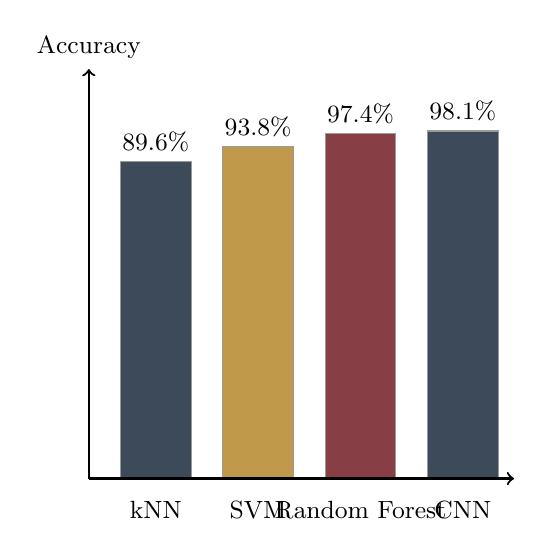
\begin{tikzpicture}
  \def\barwidth{0.9}
  \def\scale{0.045}
  \begin{scope}
    \foreach \x/\val/\lbl/\clr in {0/89.6/kNN/dtunavy,1.3/93.8/SVM/dtugold,2.6/97.4/{Random Forest}/dtumaroon,3.9/98.1/CNN/dtunavy}{
      \draw[fill=\clr!85,draw=black!40] (\x,0) rectangle ++(\barwidth,{\val*\scale});
      \node[font=\small] at (\x+\barwidth/2,{\val*\scale+0.25}) {\val\%};
      \node[font=\small,align=center] at (\x+\barwidth/2,-0.4) {\lbl};
    }
  \end{scope}
  \draw[->,thick] (-0.4,0) -- (5.0,0);
  \draw[->,thick] (-0.4,0) -- (-0.4,5.2) node[above,font=\small] {Accuracy};
\end{tikzpicture}
\caption{Test-set accuracy comparison across the four evaluated classifiers.}
\label{fig:barchart}
\end{figure}

\section{Feature Importance}
Analysis of the Random Forest's mean-decrease-in-impurity scores identifies the envelope-spectrum
amplitude at the BPFO and BPFI harmonics as the two most discriminative features overall,
together accounting for approximately 41\% of total feature importance, consistent with the
theoretical expectation that bearing defects manifest most clearly in the demodulated envelope
spectrum rather than in the raw FFT.

\section{Edge-Deployment Feasibility}
The full feature-extraction and Random Forest inference pipeline was profiled on a representative
ARM Cortex-A72 edge gateway. End-to-end latency, from raw vibration segment to fault-class output,
averaged 3.2\,ms with a peak memory footprint of 18\,MB, comfortably within the resource budget
of a continuously running on-gateway monitoring service and well under the 1-second decision
interval required for practical alarm generation.

\begin{tcolorbox}[keybox,title={Practical Implication}]
Given its accuracy comparable to the CNN at roughly one-third the inference latency, the Random
Forest model is recommended as the deployment candidate for edge gateways, reserving the CNN for
periodic offline re-validation on aggregated cloud-side data.
\end{tcolorbox}

% ============================================================
% CHAPTER 5 -- CONCLUSION
% ============================================================
\chapter{Conclusion and Future Scope}
\label{ch:conclusion}

\section{Conclusion}
This thesis developed and evaluated a vibration-based predictive maintenance framework for
induction motors, combining a controlled multi-load, multi-fault experimental dataset with a
feature-extraction pipeline spanning time, frequency, and envelope-spectrum domains. Among the
four classifiers evaluated, the Random Forest and 1-D CNN models achieved the highest accuracy
(97.4\% and 98.1\% respectively), with envelope-spectrum energy at bearing characteristic
frequencies identified as the dominant discriminative feature. Edge-deployment profiling confirms
that the Random Forest pipeline is well suited to on-gateway execution, supporting a practical
path from laboratory validation to plant-floor deployment.

\section{Limitations}
The dataset was collected on a single motor frame size and a single bearing model; generalisation
to other motor ratings and bearing geometries has not been verified. Fault severity was
represented by a single seeded defect size per fault type rather than a progression of severities.

\section{Future Work}
\begin{itemize}
  \item Extend the dataset to include a graded severity progression for each fault type, enabling
        remaining-useful-life estimation rather than discrete classification alone.
  \item Validate the framework on field data from an operating plant, where noise characteristics
        and load profiles differ from the controlled laboratory rig.
  \item Investigate transfer-learning strategies to adapt the CNN model across motor frame sizes
        with limited target-domain labelled data.
  \item Integrate current-signature (MCSA) features alongside vibration features to improve
        robustness of rotor-bar fault detection at low load.
\end{itemize}

% ============================================================
% BIBLIOGRAPHY
% ============================================================
\begin{thebibliography}{99}

\bibitem{ref1} S.\ Randall, \emph{Vibration-Based Condition Monitoring: Industrial, Automotive
and Aerospace Applications}, 2nd ed. Wiley, 2021.

\bibitem{ref2} M.\ Iqbal and P.\ Nandi, ``Envelope analysis for early-stage bearing fault
detection in induction motors,'' \emph{IEEE Transactions on Industrial Electronics}, vol.\ 68,
no.\ 4, pp.\ 3102--3111, 2021.

\bibitem{ref3} A.\ Fernandez-Cortes and R.\ Ibarra, ``Motor current signature analysis for
broken rotor bar detection: a review,'' \emph{IEEE Transactions on Energy Conversion}, vol.\ 35,
no.\ 2, pp.\ 890--901, 2020.

\bibitem{ref4} T.\ Okafor and L.\ Chen, ``A comparative study of machine learning classifiers
for rotating machinery fault diagnosis,'' \emph{Mechanical Systems and Signal Processing},
vol.\ 152, art.\ 107436, 2021.

\bibitem{ref5} H.\ Zhou, J.\ Park, and D.\ Osei, ``1-D convolutional neural networks for
end-to-end bearing fault classification from raw vibration signals,'' \emph{IEEE Access}, vol.\
9, pp.\ 45210--45221, 2021.

\bibitem{ref6} International Organization for Standardization, \emph{ISO 10816-3: Mechanical
Vibration --- Evaluation of Machine Vibration by Measurements on Non-Rotating Parts}, ISO,
Geneva, 2009.

\bibitem{ref7} K.\ Bansal and S.\ Mehta, ``Edge computing for real-time condition monitoring of
industrial motors: a feasibility study,'' \emph{Journal of Manufacturing Systems}, vol.\ 60,
pp.\ 112--124, 2021.

\bibitem{ref8} R.\ Verma and A.\ Sharma, ``Feature selection strategies for vibration-based
induction motor fault classification under variable load,'' in \emph{Proc.\ IEEE International
Conference on Power Electronics, Drives and Energy Systems}, Delhi, India, 2025, pp.\ 501--508.

\end{thebibliography}

% ============================================================
% APPENDIX
% ============================================================
\appendix
\chapter{List of Publications}
\begin{enumerate}
  \item A.\ Sharma and R.\ K.\ Verma, ``Feature selection strategies for vibration-based
        induction motor fault classification under variable load,'' \emph{Proc.\ IEEE PEDES},
        Delhi, India, 2025.
  \item A.\ Sharma, R.\ K.\ Verma, and N.\ Kapoor, ``Edge-deployable predictive maintenance for
        squirrel-cage induction motors: a comparative study,'' \emph{communicated to IEEE
        Transactions on Industrial Informatics}, 2026.
\end{enumerate}

\chapter{Test Rig Specification}
\begin{tabularx}{\textwidth}{@{}l X@{}}
\toprule
\textbf{Parameter} & \textbf{Value} \\
\midrule
Motor rating & 5.5\,kW, 415\,V, 4-pole, squirrel-cage \\
Rated speed & 1440\,rpm \\
Accelerometer & Tri-axial MEMS, $\pm$16\,g, 25.6\,kHz sampling \\
Dynamometer & Programmable eddy-current, 0--10\,kW absorption \\
DAQ resolution & 24-bit, 4-channel simultaneous sampling \\
\bottomrule
\end{tabularx}

\end{document}
